\chapter{Travulog and HTravulog}{
	% Article & books
	% - A metalanguage for SystemVerilog Transformation
	\begin{comment}
		Per realizzare un'architettura FT configurabile si devono applicare le tecniche fault tolerant a tutti i blocchi dell'IF Stage e permettere poi l'applicazione o meno delle tecniche in ciascun blocco tramite dei parametri. Si è quindi deciso di creare un metalinguaggio all'interno del SystemVerilog (SV) che permetta la creazione della nuova architettura pertendo da un template e da un modulo base. Come si vede in figura \figref{fig:TravulogFlowBlocks} Questa trasformazione viene fatta da un oggetto Python collegato al template, quando si passa il modulo base all'oggetto viene creato il nuovo modulo. Questa nuova architettura è creata sulla base del template Travulog e del modulo base, essa è quindi un layer di interfaccia che rende il vecchio modulo Fault Tolerant.
		Per permettere la conversione tramite l'oggetto Travulog è necessario avere a disposizione un oggetto che contenga tutti i dati del modulo SystemVerilog associato, si è quindi creata una nuova classe Python che effettua il parsing di un file SV contenente un modulo, questa classe è stata chiamate moddata. Come mostrato in figura  \figref{fig:TravulogFlowBlocks} il file che contiene il modulo base deve essere trasformato nel corrispondente oggetto moddata e poi passato all'oggetto Travulog che genera la nuova architettura.
	\end{comment}
	To create a configurable FT architecture it is necessary to apply fault tolerant techniques to all the blocks of the IF Stage and then allow to apply or not techniques in each block by means of parameters. It was therefore decided to create a metalanguage within the SystemVerilog (SV) that allows the creation of the new architecture starting from a template and a base module, in this way we can define a template and apply it to each block of the IF stage. As you can see in figure \figref{fig:TravulogFlowBlocks} this transformation is done by a Python object linked to the template, when you pass the base module to the object the new module is created. The new FT architecture is created on the basis of the Travulog template and the base module, it is therefore an interface layer that makes the old module Fault Tolerant. 
	To allow the conversion through the Travulog object it is necessary to have an object that contains all the data of the associated SystemVerilog base module, we have therefore created a new Python class that parses a SV file containing a module, this class has been called moddata. As shown in the figure \figref{fig:TravulogFlowBlocks} the file containing the basic module must be transformed into the corresponding moddata object and then passed to the Travulog object which generates the new architecture.
	\begin{figure}[H]
		\centering
		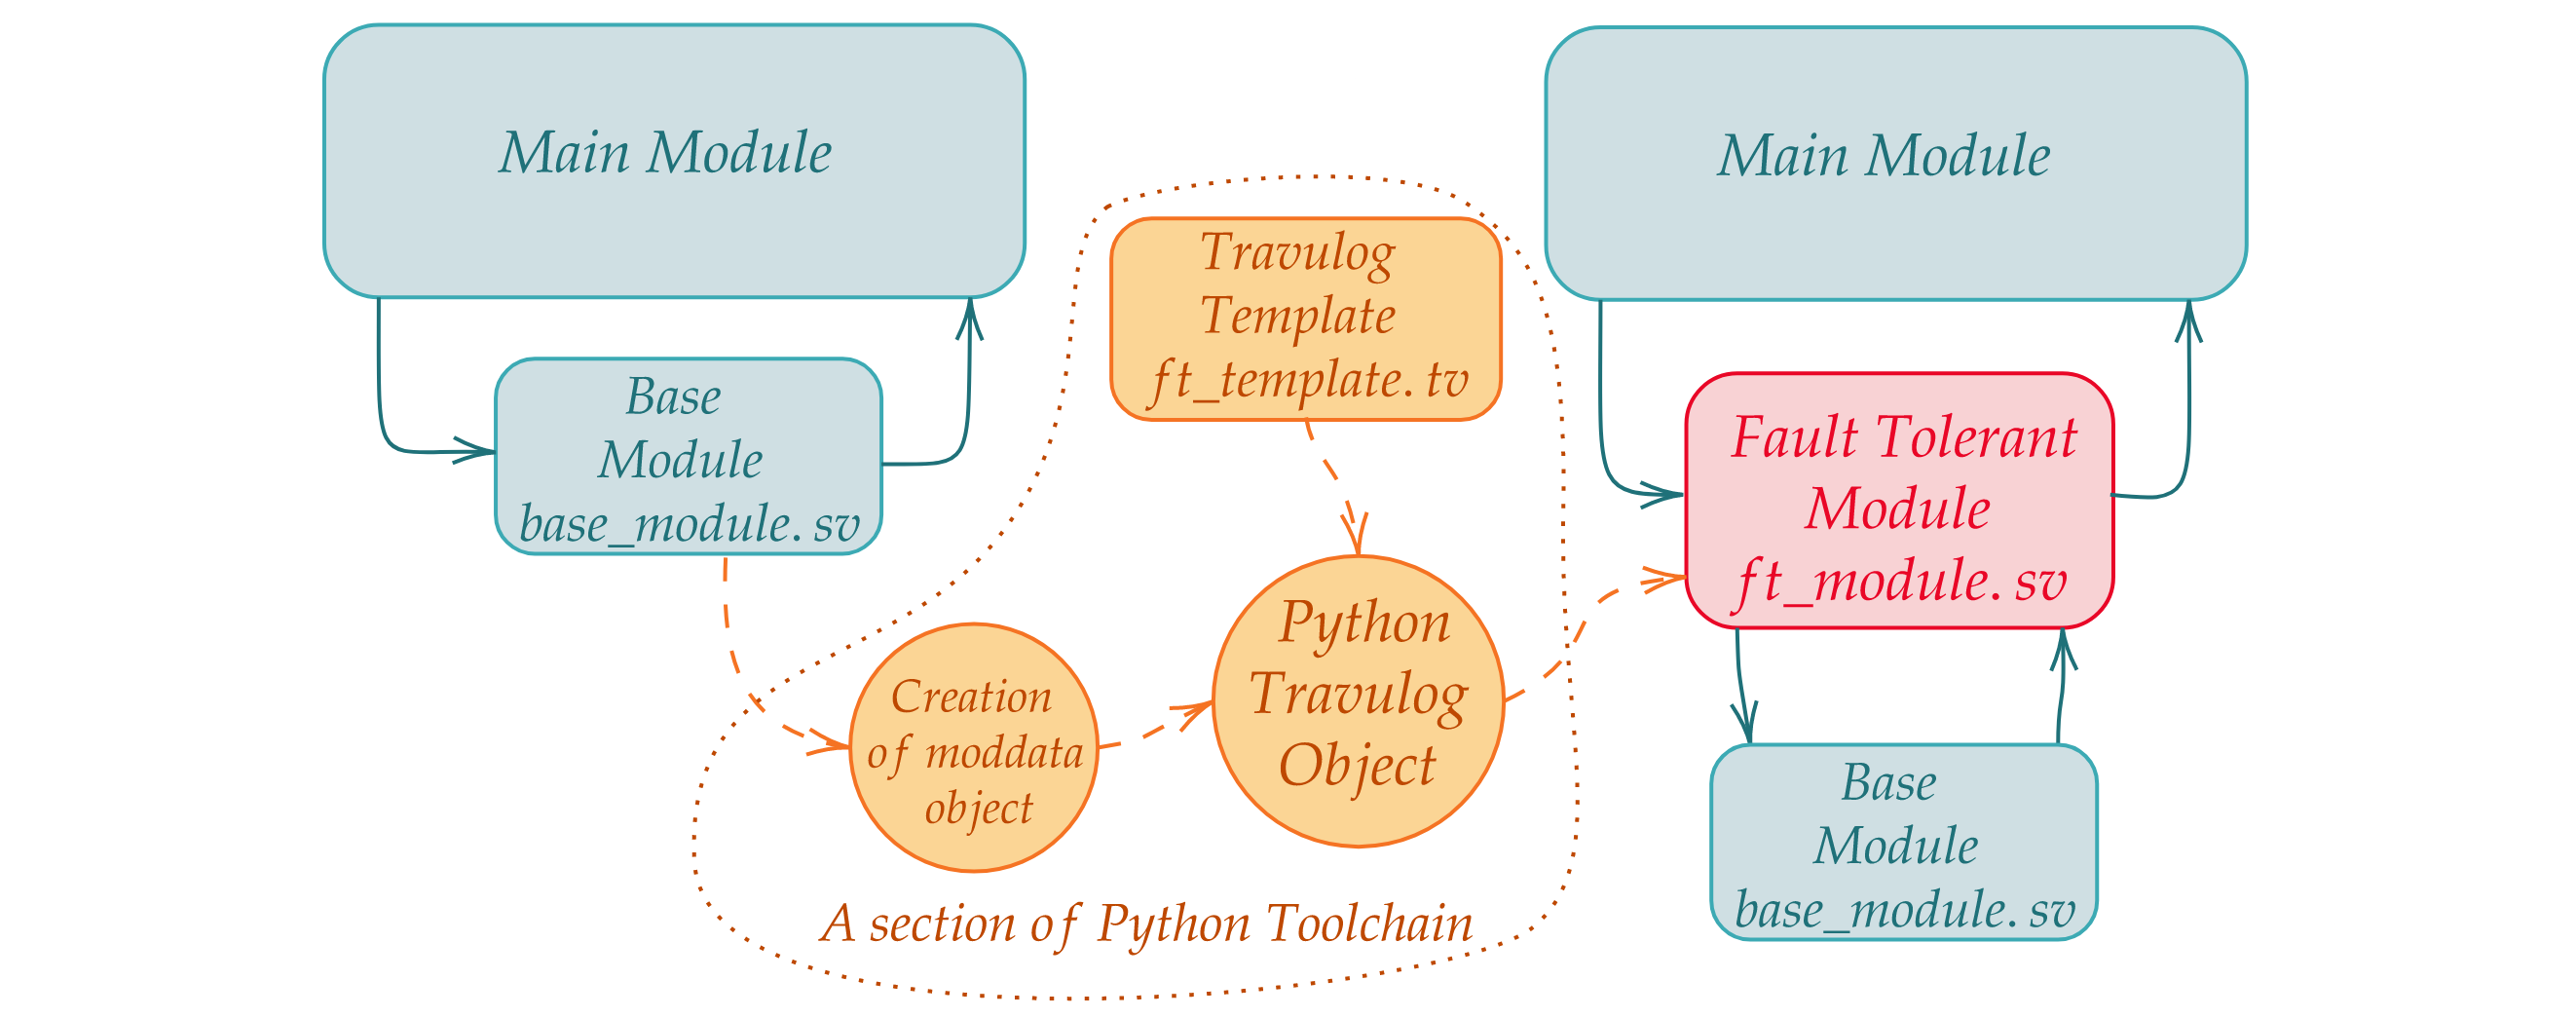
\includegraphics[scale=0.2,center]{./images/Travulog_flow_blocks.png}
		\caption{Flow diagram of architecture transformation using Travulog template}
		\label{fig:TravulogFlowBlocks}
	\end{figure} 
	\begin{comment}
		Per creare il nuovo linguaggio siamo partiti dal cv32e40p_compress_decoder (CD) fault tolerant e abbiamo creato una serie di comandi che permettono di creare il compress decoder FT da quello base. Analizzeremo ora i vari comandi Travulog facendo riferimento al compress decoder. 
	\end{comment}
	
	To create the new language we started from the fault tolerant cv32e40p\_compress\_decoder\_ft and we created a series of commands that allow us to create the FT compress decoder from the basic one. We will now analyze the various Travulog commands referring to the compress decoder, comparing pieces of code from the Travulog template and its conversion in SVerilog.
	
	
	\subsection{Declaration of ports}{
		\begin{comment}
			Nel listato \ref{lst:declTV} è presente una parte di template Travulog, questo pezzo di codice permette di generare il System Verilog del listato \ref{lst:decl:w
			SV}. di seguito vengono elencati i comandi in questa parte di template:
		\end{comment}
		In the listing \ref{lst:declTV} there is a part of the Travulog template, this piece of code allows to generate the System Verilog of the listing \ref{lst:declSV}. the commands in this part of the template are these: 
		\begin{itemize}
			\item [\textbf{PARAMETER\_DECLARATION}:] The command PARAMETER\_DECLARATION copy the parameter declaration from the BLOCK module in the new System Verilog module. BLOCK is an identifier used in the Travulog object that should be linked to a moddata object. Note that you can have multiple ID since ids are managed as a dictionary, e.g if you give {"BLOCK":moddata\_obj1, "BLOCK2":moddata\_obj2} to Travulog object you can use both BLOCK and BLOCK2 identifiers in the Travulog code.
			\item [\textbf{DECLARATION\_FOREACH}:] This command cycle on the given signals and it substitute: INOUT  with "input" or "output",  BITINIT with de bits definition and SIGNAME with the name of the signal. The first argument is the module id, the second one is the type of signal: IN for input port of the module, OUT for output, IN\_OUT for both input and output and INTERN for internal signals of the module. You can also indicate some signals to exclude by the list using "NOT sig1 sig2 ... " as you can see at line 7, indeed in the example clk and rst\_n signals are excluded since they should not be triplicated.
			This command can also be used for the declaration of internal signals and for assign statement as we see later.
			\item [\textbf{MODULE\_NAME}:] This is a parameter that is substituted with the name given to the Travulog object, it is the name of the new module.
		\end{itemize}
			
			
		\openup -0.5em
		
		\begin{parcolumns}[colwidths={1=0.54\textwidth}, distance=0.5em]{2}
			\colchunk{%
				\begin{lstlisting}[basicstyle=\ttfamily\scriptsize, language=Verilog, caption=Travulog Code, label=lst:declTV]
module MODULE_NAME
	
	PARAMETER_DECLARATION BLOCK

(
	// compressed decoder input output
	DECLARATION_FOREACH BLOCK IN_OUT NOT clk rst_n
		INOUT logic [2:0]BITINIT SIGNAME,
	END_DECLARATION_FOREACH

	
	input logic clk,
	input logic rst_n,  
	
	// fault tolerant state
	input logic [2:0] set_broken_i,
	output logic [2:0] is_broken_o,
	output logic err_detected_o,
	output logic err_corrected_o
);
				\end{lstlisting}
			}
			\colchunk{%
				\begin{lstlisting}[basicstyle=\ttfamily\scriptsize, language=Verilog, numbers=none, caption=SVerilog code derived, label=lst:declSV]
module cv32e40p_compressed_decoder_ft
#(
	parameter FPU = 0
)
(
	// compressed decoder input output
	input  logic [2:0] [31:0] instr_i,
	output logic [2:0] [31:0] instr_o,
	output logic [2:0] is_compressed_o,
	output logic [2:0] illegal_instr_o,
	
	input logic clk,
	input logic rst_n,    
	
	// fault tolerant state
	input logic [2:0] set_broken_i,
	output logic [2:0] is_broken_o,
	output logic err_detected_o,
	output logic err_corrected_o
);
				\end{lstlisting}
			}
		\end{parcolumns}
	
		\openup +0.5em
		
		
	}% end Declaration of ports
		\subsection{Internal signals and assign}{
		In the following listings you can see the continuation of the previous ports definition, the first "declaration\_foreach" create the signals that connect the three block outputs to the voter while the second creates block error signals. In the last two lines there is the compound parameter "SIG\_NUM-BLOCK-OUT" inside the square bracket,  this parameter is substituted in the right listing with the number (SIG\_NUM) of output ports (OUT) of the module (BLOCK) minus one, anyway instead of OUT you can use IN, PARAM, INTERN or IN\_OUT in order to have the correct signals number.
		
		\openup -0.5em
		
		\begin{parcolumns}[colwidths={1=0.5\textwidth}, distance=0.5em]{2}
			\colchunk{%
				\begin{lstlisting}[basicstyle=\ttfamily\scriptsize, language=Verilog, caption=Travulog Code, label=lst:internTV]
// Signals out to each compressed 
// decoder block to be voted
DECLARATION_FOREACH BLOCK OUT 
logic [2:0]BITINIT SIGNAME_to_vote ;
END_DECLARATION_FOREACH

// Error signals
DECLARATION_FOREACH BLOCK OUT 
logic [2:0] SIGNAME_block_err ; 
END_DECLARATION_FOREACH

// Signals that use error signal to 
// find if there is one error on each 
// block, it is the or of previous signals
logic [2:0] block_err_detected;
logic [SIG_NUM-BLOCK-OUT:0] err_detected;
logic [SIG_NUM-BLOCK-OUT:0] err_corrected;
				\end{lstlisting}
			}
			\colchunk{%
				\begin{lstlisting}[basicstyle=\ttfamily\scriptsize, language=Verilog, numbers=none, caption=SVerilog code derived, label=lst:internSV]
// Signals out to each compressed 
// decoder block to be voted
logic [2:0] [31:0] instr_o_to_vote ;
logic [2:0] is_compressed_o_to_vote ;
logic [2:0] illegal_instr_o_to_vote ;

// Error signals
logic [2:0] instr_o_block_err ;
logic [2:0] is_compressed_o_block_err ;
logic [2:0] illegal_instr_o_block_err ;

// Signals that use error signal to 
// find if there is one error on each 
// block, it is the or of previous signals
logic [2:0] block_err_detected;
logic [2:0] err_detected;
logic [2:0] err_corrected;
				\end{lstlisting}
			}	
		\end{parcolumns}

		\openup +0.5em
	
	} % end Internal signals and assign
	\subsection{Instance}{
			\begin{comment}
				Per poter creare una nuova instanza da un blocco esistente è stato creato il comando INSTANCE mostrato nel listing \ref{lst:instance1TV}. 
			\end{comment}
						
			\openup -0.5em
		
			\begin{parcolumns}[colwidths={1=0.5\textwidth}, distance=0.5em]{2}
			\colchunk{%
				\begin{lstlisting}[basicstyle=\ttfamily\scriptsize, language=Verilog, caption=Travulog Code, label=lst:instance1TV]
INSTANCE BLOCK BLOCK_MODNAME_no_ft
	PARAM=PARAM
	IF clk rst_n IN=IN
	IN= IN[0]
	OUT = OUT[0]
END_INSTANCE



		
		
		
		
		
				\end{lstlisting}
			}
			\colchunk{%
				\begin{lstlisting}[basicstyle=\ttfamily\scriptsize, language=Verilog, numbers=none, caption=SVerilog code derived, label=lst:instance1SV]
cv32e40p_compressed_decoder
#(
	.FPU (FPU)
)
compressed_decoder_no_ft
(
	// Input ports of compressed_decoder_no_ft
	.instr_i                (  instr_i[0]),
	
	// Output ports of compressed_decoder_no_ft
	.instr_o        (  instr_o[0]),
	.is_compressed_o(  is_compressed_o[0] ),
	.illegal_instr_o(  illegal_instr_o[0] )
);		
				\end{lstlisting}
			}	
		\end{parcolumns}
	
		\openup +0.5em
	

	} % end instance
	\section{Travulog}{
		
	
	}% end RISCV 32bit ISA 

	\section{Hidden Travulog}{
	
	}% end of Architecture of CV32E40P
	
	\section{V}{
		
	}% end of Verification of CV32E40P core

	\section{CV32E40P core in Pulpissimo}{
		
	}% end of CV32E40P core in Pulpissimo

}
